\documentclass{article}

\usepackage{amsthm}
\usepackage{epsfig}
\usepackage{graphicx}
\usepackage{color}
\usepackage{url}
\usepackage{amsfonts}
\usepackage[utf8]{inputenc}
\usepackage{amsmath}
\usepackage{xspace}
\usepackage{amssymb}
\usepackage{amstext}
\usepackage{hyperref}
\usepackage[english]{babel}
\usepackage{times}
\usepackage{mathtools}
\usepackage[T1]{fontenc}
\usepackage{rotating}
\usepackage{tikz,tkz-tab}



\addtolength{\tabcolsep}{1pt}

%------------------------------------------------------------------------- 



\begin{document}

\title{\LaTeX pour les noobs}
\author{Nvoskerjen, Chataninho}
\maketitle


\vspace{40mm}





\pagebreak

\section{Introduction}


\LaTeX permet à l'auteur de ne pas s'inquiéter de l'apparence de son document et de se concentrer sur le fond et non la forme. Cependant, \LaTeX est principalement utilisé pour des publications scientifiques. Il faut ainsi souvent connaître les codes pour faire certaines formules. C'est pourquoi nous avons commencé un projet qui consiste à recenser tous les codes intéressants et à permettre une recherche rapide dans ce document.
\section{Couleur, alignement}

\section{rotation}
nécessite \textbackslash usepackage\{rotating\}
\begin{turn}{30}
toto
\end{turn}
\section{Faire une énumération}
\begin{itemize}
\item The first item
\item The second item
\item The third\ldots
\end{itemize}

\begin{enumerate}
\item The first item
\item The second item
\item The third\ldots
\end{enumerate}

\begin{description}
\item[First] The first item
\item[Second] The second item
\item[Third] The third\ldots
\end{description}

\begin{description}
\item[First] \hfill \\
The first item
\item[Second] \hfill \\
The second item
\item[Third] \hfill \\
The third\ldots
\end{description}
\section{Tableau}
Tableau de Variation :\\
nécessite \textbackslash usepackage\{tikz,tkz-tab\}\\
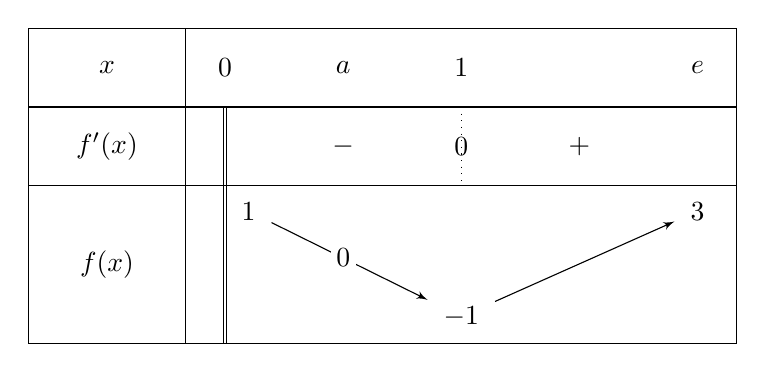
\begin{tikzpicture}
\tkzTabInit{$x$/1,$f'(x)$/1,$f(x)$/2}{$0$, $1$, $e$}
\tkzTabLine{d,-,z,+}
\tkzTabVar{D+/$1$,-/$-1$,+/$3$}
\tkzTabVal{1}{2}{0.5}{$a$}{$0$}
\end{tikzpicture}

\section{Lettres}
Lettre double barre (Set) : \$\textbackslash mathbb\{Lettre\}\$ :\\
$\mathbb{A,B,C,D,E,F,G,H,I,J,K,L,M,N,O,P,Q,R,S,T,U,V,W,X,Y,Z}$\\
Lettre ronde : \$\textbackslash mathcal\{Lettre\}\$ :\\
$\mathcal{A,B,C,D,E,F,G,H,I,J,K,L,M,N,O,P,Q,R,S,T,U,V,W,X,Y,Z}$\\
Lettre fraktur : \$\textbackslash mathfrak\{Lettre\}\$ :\\
$\mathfrak{A,B,C,D,E,F,G,H,I,J,K,L,M,N,O,P,Q,R,S,T,U,V,W,X,Y,Z}$\\
\emph{a,b,c,d,e,f,g,h,i,j,k,l,m,n,o,p,q,r,s,t,u,v,w,x,y,z}\\
Alphabet grec minuscule :\\
\textbackslash alpha, \textbackslash beta, \textbackslash gamma, \textbackslash delta, \textbackslash epsilon, \textbackslash eta, \textbackslash theta, \textbackslash iota, \textbackslash kappa, \textbackslash lambda, \textbackslash mu, \textbackslash nu, \textbackslash xi, \textbackslash o, \textbackslash pi, \textbackslash rho, \textbackslash sigma, \textbackslash tau, \textbackslash upsilon, \textbackslash phi, \textbackslash chi, \textbackslash psi, \textbackslash omega\\
$\alpha, \beta, \gamma, \delta, \epsilon, \eta, \theta, \iota, \kappa, \lambda, \mu, \nu, \xi, \o, \pi, \rho, \sigma, \tau, \upsilon, \phi, \chi, \psi, \omega$\\

Alphabet grec majuscule  : cf l'alphabet grec en minuscule en changeant la première lettre en une majuscule.
\section{Calcul de base}

indice : x\_y : $x_y$\\
exposant, puissance : x\^{ }y : $x^y$\\
fraction : \textbackslash frac\{x\}\{y\} : $\frac{x}{y}$\\
racine : \textbackslash sqrt \{x\} : $\sqrt{X}$\\
binome de Newton : \textbackslash binom\{n\}\{k\} : $\binom{n}{k}\\
$
Intégration\\
Dérivation\\
Dérivation partielle\\
vecteur : \textbackslash overrightarrow\{AB\} $\overrightarrow{AB}$\\
angle \textbackslash widehat\{abc\} : $\widehat{abc}$\\
$\overbrace{abc}$

\section{Intersection/Union}
$
\bigcup_{i=1}^n A_i\\
\bigcap_{i=1}^n A_i$
\section{Calcul Matricielle, Matrice}


\section{Limite, flèche}
texte en dessous d'une flèche :\\
u\_n\textbackslash underset\{n\textbackslash to+\textbackslash infty\}\{\textbackslash longrightarrow\} \textbackslash ell  $u_n\underset{n\to+\infty}{\longrightarrow}\ell$\\
    \\
    texte au dessus d'une flèche :\\
    u\_n\textbackslash overset\{n\textbackslash to+\textbackslash infty\}\{\textbackslash longrightarrow\}\textbackslash ell
$u_n\overset{n\to+\infty}{\longrightarrow}\ell\\
a \xleftrightarrow[under]{over} b\\
A \xLeftarrow[under]{over} B\\
B \xRightarrow[under]{over} C\\
%
C \xLeftrightarrow[under]{over} D\\
%
D \xhookleftarrow[under]{over} E\\
%
E \xhookrightarrow[under]{over} F\\
%
F \xmapsto[under]{over} G\\
%
H \xrightharpoondown[under]{over} I\\
%
I \xrightharpoonup[under]{over} J\\
%
J \xleftharpoondown[under]{over} K\\
%
K \xleftharpoonup[under]{over} L\\
%
L \xrightleftharpoons[under]{over} M\\
%
M \xleftrightharpoons[under]{over} N
$
\section{Logique}
$\forall
\exists$

\section{Comparateur}

\section{Géométrie}

\section{Graphe}
Graphe
Arbre


\section{\'Ecrire une équation}
définie en plusieurs morceaux :\\
$
u(x) =
\begin{cases}
\exp{x} & \text{if } x \geq 0 \\
1 & \text{if } x < 0
\end{cases}
$
\section{Faire une bibliographie}

\end{document}
